\section{SAT Model}

\subsection{Decision Variables}
To encode the Sports Tournament Scheduling (STS) problem, we define the following decision variables:
\begin{enumerate}
    \item $\text{\textbf{match\_period\_vars}}[i,j,p] \in \{\mathrm{True}, \mathrm{False}\}$, for all $i,j \in T$ with $i < j$, and $p \in P$. \\
    This variable is true if and only if team $i$ plays against team $j$ during period $p$. The week for each match-up $(i,j)$ is precomputed (see Section~\ref{CircleMatching}) and fixed.
    
    \item $\text{\textbf{home\_vars}}[i,j] \in \{\mathrm{True}, \mathrm{False}\}$, for all $i,j \in T$ with $i < j$. \\
    This variable is true if and only if team $i$ plays at home against team $j$.
\end{enumerate}

\subsection{Objective Function}
The implemented objective function is defined in Section~\ref{obj_var}.

Since SAT solvers handle only boolean variables, we solve this optimization problem via a \emph{binary search} on the maximum allowed imbalance $k$.

For each team $t \in T$, the number of home games $H_t$ is defined as
\[
H_t = \sum_{\substack{(i,j) \in \text{pair\_to\_week} \\ p \in P}}
\begin{cases}
1 & \text{if } t = i \land \text{match\_period\_vars}_{i,j,p} \land \text{home\_vars}_{i,j} \\
1 & \text{if } t = j \land \text{match\_period\_vars}_{i,j,p} \land \neg \text{home\_vars}_{i,j} \\
0 & \text{otherwise}
\end{cases}
\]

To enforce that the home-away imbalance for each team $t$ does not exceed $k$, we use two pseudo-boolean constraints. For a given $k$, the constraints are:
\begin{enumerate}
    \item $H_t \ge \text{lower\_bound}$, where $\text{lower\_bound} = \left\lceil \frac{\text{w} - k}{2} \right\rceil$,
    \item $H_t \le \text{upper\_bound}$, where $\text{upper\_bound} = \left\lfloor \frac{\text{w} + k}{2} \right\rfloor$.
\end{enumerate}
These bounds ensure that the number of home games for each team respects the maximum imbalance $k$. Since the maximum number of matches a team can play is $|W|$, which is odd, then the optimal value we want to achieve is exactly $k=1$. For other details, see section~\ref{validation}.


\subsection{Constraints}
Thanks to the \emph{circle method}, some constraints are inherently satisfied (see Section~\ref{CircleMatching}).
This reduces the constraints needed, leaving the solver to decide only the specific period for each match $(i,j)$,  where $(i,j) \in \mathcal{M}_w$ ($\mathcal{M}_w$ is the set of matches scheduled in week $w \in W$). In particular, we implemented the following constraints:

\textbf{Each match is assigned to exactly one period:}
\[
\forall (i,j) \in \text{pair\_to\_week}: \quad \sum_{p \in P} \text{match\_period\_vars}_{i,j,p} = 1
\]

\textbf{Each period in each week contains exactly one match:}
\[
\forall w \in W, \forall p \in P: \quad \sum_{(i,j) \in \mathcal{M}_w} \text{match\_period\_vars}_{i,j,p} = 1
\]

\textbf{Each team plays at most twice in the same period:}
\[
\forall t \in T, \forall p \in P: \quad \sum_{\substack{(i,j) \in \text{pair\_to\_week} \\ t \in \{i,j\}}} \text{match\_period\_vars}_{i,j,p} \leq 2
\]

\subsubsection*{Symmetry Breaking Constraints}
To reduce redundant search caused by symmetric solutions, we experimented with several symmetry breaking (SB) constraints.

\textbf{SB1: Match between teams 0 and $n-1$ is in the first period:}
\[
\text{match\_period\_vars}_{0,n-1,0} = 1
\]
This fixes the match between the pivot team $n-1$ and team 0 in period 0, breaking rotational symmetry.

We also investigated two further constraints, which are commented in the code and reported here only for completeness. Since they introduced additional complexity that outweighed any potential benefits, they were not considered in the final results.

\textbf{SB2: Team 0's home/away pattern is fixed:} This enforces a fixed home/away assignment for team 0.

\textbf{SB3: Lexicographical ordering of matches in week 0:} This constraint enforces a lexicographical order on the period assignments of matches in week 0.


\subsubsection*{Encoding Methods}
We implemented all the encoding methods covered in class:

\begin{enumerate}
    \item For the \textit{exactly-one} constraint: Pairwise, Bitwise, Sequential, and Heule encodings.
    \item For the \textit{at-most-$k$} constraint: Pairwise, Sequential, and Totalizer encodings.
\end{enumerate}

Additionally, we employed the \textbf{Totalizer encoding}~\cite{bailleux2003} to efficiently model cardinality constraints. This encoding builds a balanced binary tree of adders and is known for scalability and efficiency in SAT formulations. It introduces $O(n \log n)$ auxiliary variables and up to $O(n^2)$ clauses in the worst case.

\subsection{Validation}
\label{validation}
The model was implemented in Python using Z3's API. 


In the following, we present tables and plots to compare the Z3 model using different encoding techniques (used for both optimization and decision versions), both with and without symmetry breaking constraints:

\begin{enumerate}
\item Pairwise + Pairwise encodings  (p-p in the Table)
\item Heule + Sequential encodings   (h-s in the Table)
\item Heule + Totalizer encodings    (h-t in the Table)
\end{enumerate}


\subsubsection{Experimental Results (Decision version)}
As shown in Table~\ref{tab:sat-results-dec}, even a simple symmetry breaking (SB) constraint can effectively guide the solver, leading to noticeably faster search times.

\begin{table}[H]
    \centering
    \small % Riduce la dimensione del testo nella tabella
    \caption{Runtime in seconds for the SAT (decision) version using the Z3 solver, with and without symmetry breaking (SB).}
    \label{tab:sat-results-dec}
    \centerline{
    \begin{tabular}{ccccccc}
        \toprule
        \textbf{N} & \textbf{p-p + SB} & \textbf{p-p w/out SB} & \textbf{h-s + SB} & \textbf{h-s w/out SB} & \textbf{h-t + SB} & \textbf{h-t w/out SB} \\ 
        \midrule
        12 & 1.0 & 1.0 & 0.0 & 0.0 & 0.0 & 0.0 \\
        14 & 3.0 & 2.0 & 0.0 & 0.0 & 1.0 & 0.0 \\
        16 & 4.0 & 26.0 & 7.0 & 3.0 & 5.0 & 10.0 \\
        18 & 17.0 & 80.0 & 8.0 & 11.0 & 7.0 & 15.0 \\
        20 & N/A & N/A & 79.0 & N/A & 150.0 & 151.0\\
        \bottomrule
    \end{tabular}
    }
\end{table}


\subsubsection{Experimental Results (Optimization version)}
As shown in Table \ref{tab:sat_results_opt}, the results confirm the expected performance of the encodings. The Heule + Totalizer combination generally proved to be very efficient, particularly for larger instances. Conversely, the Pairwise + Pairwise approach, known for its larger number of clauses, was the slowest.

Generally, except for some rare cases, the SB constraint proved effective at guiding the solver to an optimal solution faster, significantly reducing the search space.

The table also shows that all tested configurations successfully found an \textbf{optimal solution} for $N\le18$. 

\begin{table}[H]
    \centering
    \caption{SAT results. Results are of the type "time\textbar\textbf{optimal value}" or "time\textbar suboptimal value".}
    \label{tab:sat_results_opt}
    \small
    \centerline{
    \begin{tabular}{ccccccc}
        \toprule
        \textbf{N} & \textbf{p-p + SB} & \textbf{p-p w/out SB} & \textbf{h-s + SB} & \textbf{h-s w/out SB} & \textbf{h-t + SB} & \textbf{h-t w/out SB} \\ 
        \midrule
        10  & 1\textbar\textbf{1}  & 1\textbar\textbf{1}  & 0\textbar\textbf{1}  & 0\textbar\textbf{1}  & 0\textbar\textbf{1}  & 0\textbar\textbf{1}  \\ 
        12  & 2\textbar\textbf{1} & 3\textbar\textbf{1} & 0\textbar\textbf{1} & 1\textbar\textbf{1} & 1\textbar\textbf{1} & 1\textbar\textbf{1} \\ 
        14  & 7\textbar\textbf{1}  & 7\textbar\textbf{1}  & 3\textbar\textbf{1}  & 3\textbar\textbf{1}  & 2\textbar\textbf{1}  & 5\textbar\textbf{1}  \\ 
        16 & 46\textbar\textbf{1} & 35\textbar\textbf{1} & 37\textbar\textbf{1} & 25\textbar\textbf{1} & 36\textbar\textbf{1} & 34\textbar\textbf{1} \\ 
        18  & 207\textbar\textbf{1} & 292\textbar\textbf{1} & 143\textbar\textbf{1} & 160\textbar\textbf{1} & 150\textbar\textbf{1} & 98\textbar\textbf{1} \\ 
        20  & N/A & N/A & 300\textbar{5} & N/A & 300\textbar{10} &  N/A\\ 
        \bottomrule
    \end{tabular}
    }
\end{table}


\begin{figure}[H]
    \centering
    \begin{subfigure}{0.75\linewidth}
        \centering
        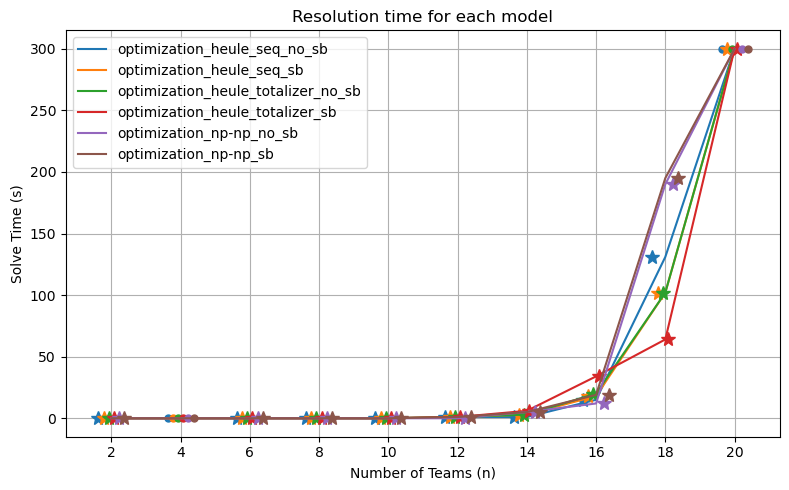
\includegraphics[width=\linewidth]{imgs/output.png}
        \caption{Resolution time}
    \end{subfigure}
    \caption{Runtimes for the optimization version of the Sports Tournament Scheduling (STS) problem. Data points are marked to indicate the solution status: a star ($\star$) indicates that a solution (optimal or sub-optimal) was found, while a circle ($\bullet$) indicates that no solution was found within the time limit.}
\end{figure}








